
\documentclass[12pt,a4paper]{article}

\usepackage[utf8]{inputenc}
\usepackage[T1]{fontenc}
\usepackage[spanish,es-nodecimaldot]{babel}

\usepackage{geometry}
\geometry{margin=2.5cm}
\usepackage{setspace}
\onehalfspacing
\usepackage{graphicx}
\usepackage{float}
\usepackage{booktabs}
\usepackage{longtable}
\usepackage{hyperref}
\usepackage{csquotes}

\usepackage[
    backend=biber,
    style=ieee,
    sorting=none
]{biblatex}

\addbibresource{../referencias/referencias.bib}
\graphicspath{{../figuras/}{../anexos/}}

\begin{document}


\begin{titlepage}
    \centering

    {\Large UNIVERSIDAD TÉCNICA ESTATAL DE QUEVEDO\par}
    \vspace{0.5cm}

    {\large Facultad de Ciencias de la Computación\par}
    {\large Carrera de Software\par}

    \vspace{1.5cm}

    {\large Asignatura: Aplicaciones Distribuidas\par}
    {\large Código de actividad: TA-IND-01\par}

    \vspace{1.5cm}

    {\LARGE\bfseries
    Análisis crítico comparativo de Syncthing y Unison\par}

    \vspace{1.5cm}

    {\large Estudiante: Steffanny del Rocío Loor Suárez\par}
    {\large Paralelo: B\par}
    {\large Docente: Guerrero Ulloa Gleiston Ciceron\par}

    \vfill

    {\small Repositorio GitHub:\par}
    {\small
    \url{https://github.com/SteffannyLoorSuarez1/TA-IND-01}
    \par}

    \vspace{1cm}

    {\large Quevedo, Ecuador\par}
    {\large 14 de noviembre de 2026\par}

\end{titlepage}

\begin{abstract}
    En este informe se presenta un análisis crítico de Syncthing como sistema distribuido para la sincronización de archivos 
    entre dispositivos. Se estudia su arquitectura, comunicación entre nodos y su comportamiento frente a interrupciones, relacionando estos 
    aspectos con las transparencias de distribución, el teorema CAP, PACELC y la tolerancia a fallos. También se compara Syncthing con Unison para identificar 
    diferencias en sus mecanismos de sincronización y recuperación.
    Para complementar el análisis, se realizaron dos experimentos con Syncthing v2.1.7 en una computadora (con sistema operativo Windows), utilizando 
    dos procesos independientes y carpetas locales diferentes. En el primero, se creó un archivo en el Nodo A y se comprobó su sincronización con el Nodo B mediante la comparación de hashes SHA-256. 
    En el segundo, se apagó el Nodo B y se modificó el archivo en el Nodo A. Durante la interrupción, los hashes fueron diferentes, pero volvieron a coincidir después de restablecer la conexión.
    Los resultados muestran que Syncthing logró recuperar la sincronización después de interrumpir uno de sus procesos. Sin embargo, como ambos nodos se ejecutaron en una misma computadora, no 
    se evaluó su comportamiento ante el fallo de equipos físicos diferentes.
\end{abstract}

\newpage
\section{Introducción}

Mantener archivos actualizados entre diferentes dispositivos es una necesidad frecuente para personas que trabajan o estudian utilizando más de una computadora. 
Syncthing es una herramienta de código abierto que permite sincronizar carpetas sin depender de un servicio central de almacenamiento en la nube \cite{syncthingFAQ}.
Esta herramienta puede ser utilizada por usuarios particulares, estudiantes y pequeños equipos de trabajo que necesitan conservar 
copias de sus archivos en distintos dispositivos. Su funcionamiento permite estudiar aspectos de los sistemas distribuidos, como el intercambio de información, la replicación y la recuperación después de interrupciones.
Se eligió Syncthing porque permite observar estos mecanismos mediante pruebas prácticas. En este informe se analiza su arquitectura, sus mecanismos de comunicación 
y su comportamiento ante la desconexión temporal de un nodo. Además, se compara con Unison para identificar diferencias entre sus enfoques de sincronización.

\section{Descripción del sistema distribuido}

Syncthing permite compartir carpetas entre dispositivos previamente autorizados. 
Cada participante conserva sus propios archivos y puede recibir modificaciones realizadas en otros dispositivos que comparten la misma carpeta. El sistema identifica los cambios y coordina la actualización de las copias cuando los dispositivos pueden comunicarse \cite{syncthingFAQ}.
Una característica importante es que los archivos permanecen almacenados en los dispositivos participantes.
Esto permite que cada uno conserve una copia local y pueda acceder a ella incluso cuando otro dispositivo no está conectado. Sin embargo, los cambios realizados durante una desconexión no se reflejan inmediatamente en las demás copias \cite{syncthingFAQ}.
La sincronización depende de la configuración de las carpetas y de los permisos establecidos para los dispositivos participantes. Por ello, Syncthing no debe confundirse con un sistema de 
edición colaborativa en tiempo real: su propósito principal es mantener sincronizadas las copias de los archivos, y las modificaciones simultáneas pueden producir conflictos que deben resolverse \cite{syncthingFAQ}.

\section{Arquitectura y comunicación entre procesos}

\subsection{Modelo de arquitectura}

Una arquitectura \textit{peer-to-peer} (P2P) es un modelo de red distribuida en el que los nodos pueden 
intercambiar datos y recursos entre sí, sin depender necesariamente de un servidor central para todas las operaciones. 
En este modelo, la disponibilidad de los participantes y la conectividad influyen en el intercambio y la replicación de información \cite{samimi2025}.

Syncthing utiliza una arquitectura P2P para mantener sincronizadas las carpetas de los dispositivos autorizados. 
Cada dispositivo ejecuta un proceso que administra sus archivos y establece conexiones con otros nodos. 
Para facilitar la comunicación, Syncthing utiliza identificadores de dispositivo y puede apoyarse en servicios de descubrimiento. Cuando una conexión directa no es posible, también puede utilizar servidores de retransmisión, 
que permiten intercambiar información sin funcionar como un almacenamiento central de los archivos \cite{syncthingFAQ,syncthingRelay}.

\subsection{Arquitectura del entorno experimental}

Para las pruebas se configuraron dos procesos independientes de Syncthing v2.1.7 en una computadora con sistema operativo Windows. 
El Nodo A y el Nodo B utilizaron directorios de configuración y carpetas locales diferentes. Ambos compartieron una carpeta identificada como \texttt{prueba-sync}, lo que permitió estudiar la comunicación entre dos instancias del sistema.

\begin{figure}[H]
    \centering
    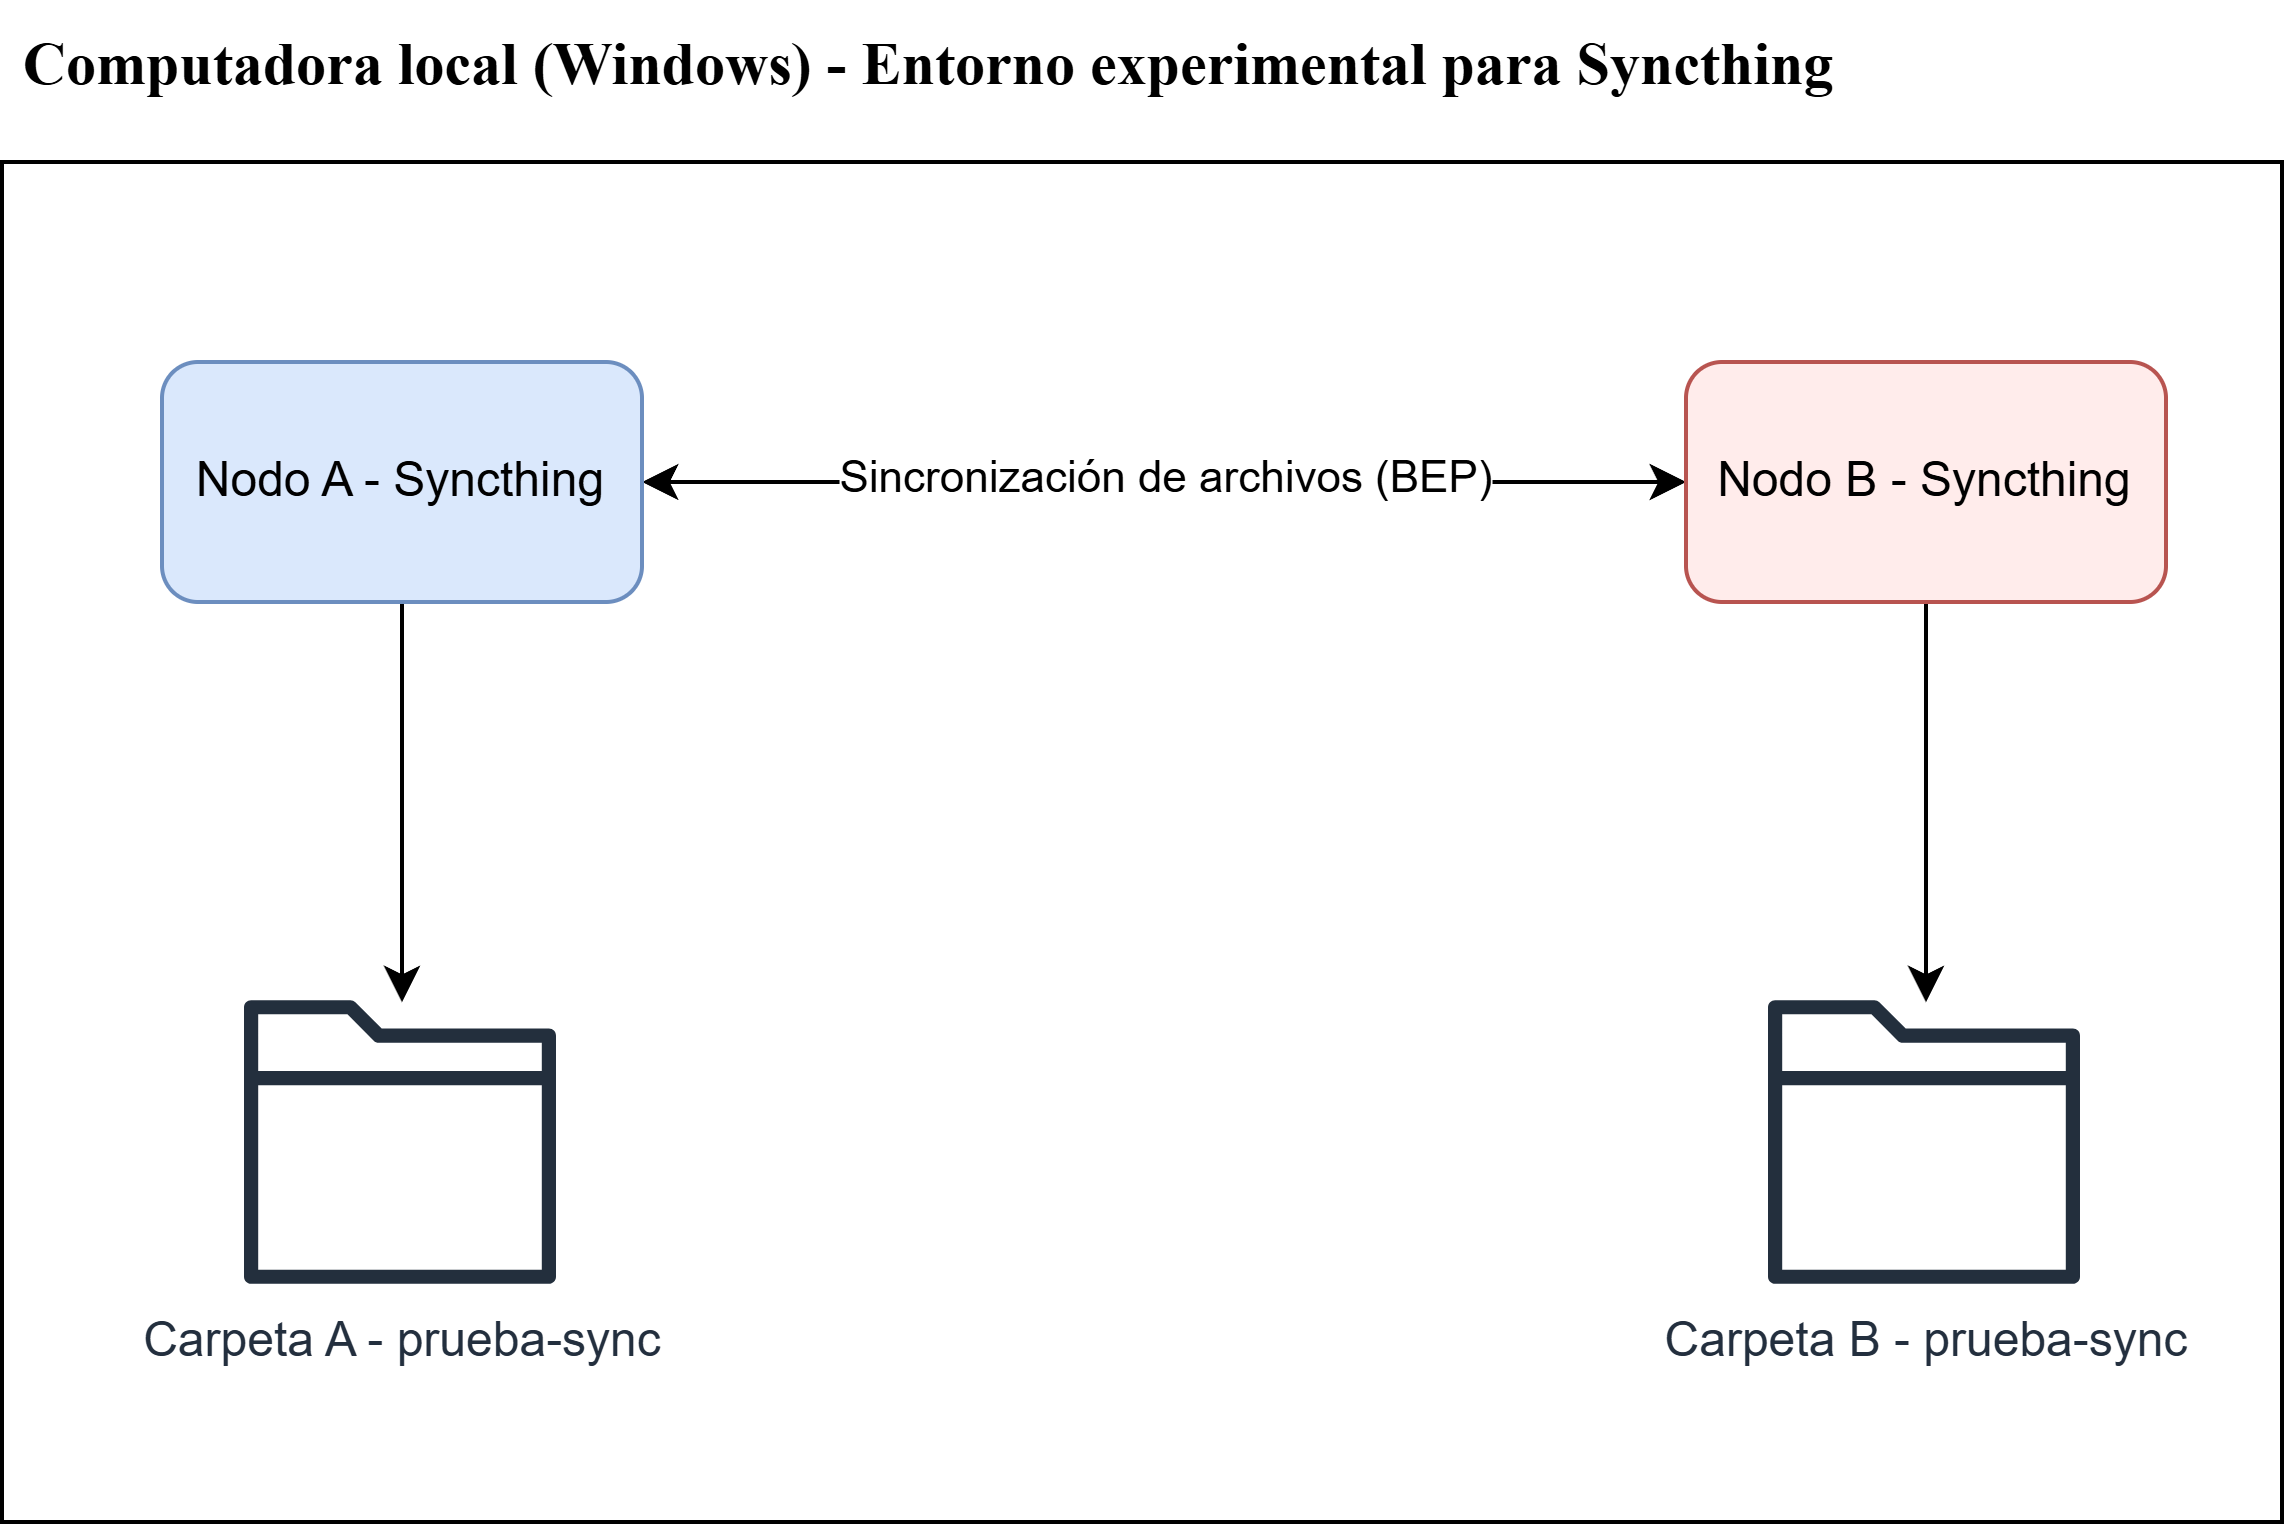
\includegraphics[width=0.90\textwidth]{arquitectura-syncthing.png}
    \caption{Arquitectura del entorno experimental de Syncthing con dos procesos independientes en una computadora Windows.}
    \label{fig:arquitectura-syncthing}
\end{figure}

Como se observa en la Figura~\ref{fig:arquitectura-syncthing}, cada proceso administra una carpeta local y se comunica con el otro para intercambiar información. Aunque funcionan como instancias independientes, ambos dependen de una misma computadora. Por tanto, esta configuración permite analizar la comunicación entre procesos, pero no representa una red de dos equipos físicos independientes.

\subsection{Comunicación y protocolo BEP}

Syncthing utiliza el protocolo \textit{Block Exchange Protocol} (BEP) para intercambiar información 
sobre los archivos compartidos. Mediante este protocolo, los nodos anuncian los archivos que conocen, informan sobre sus modificaciones y solicitan los bloques necesarios para actualizar sus copias \cite{syncthingBEP}.
Entre los mensajes definidos por BEP se encuentran \textit{Index} e \textit{Index Update}, 
utilizados para comunicar información sobre los archivos; \textit{Request}, para solicitar bloques de datos; y \textit{Response}, para responder a esas solicitudes. Estos mensajes permiten distinguir el intercambio de metadatos del intercambio del contenido de los archivos \cite{syncthingBEP}.
La comunicación es bidireccional, ya que ambos nodos pueden anunciar modificaciones y solicitar bloques. Aunque BEP utiliza mensajes de solicitud y respuesta, no constituye una implementación de RPC tradicional, 
sino un protocolo específico para la sincronización entre pares \cite{syncthingBEP}.
Desde la perspectiva del usuario, la sincronización no requiere que todos los dispositivos permanezcan conectados al mismo tiempo. Los archivos pueden modificarse localmente y los cambios pendientes pueden propagarse cuando se restablece la comunicación \cite{syncthingFAQ}. 
Este comportamiento se analizará posteriormente mediante las evidencias del experimento de interrupción y recuperación.
El diagrama representa únicamente los componentes configurados durante las pruebas. No se incluyeron servidores externos de descubrimiento ni de retransmisión porque no se verificó que participaran en la comunicación entre las dos instancias locales.

\section{Propiedades y transparencias de distribución}

\section{Consistencia, disponibilidad y tolerancia a fallos}

\section{Experimentos y análisis de resultados}

\section{Comparación crítica con Unison}

\section{Conclusiones}

\printbibliography[title={Referencias bibliográficas}]

\appendix

\section{Bosquejo inicial de arquitectura}

\section{Evidencias de ejecución y experimentación}

\end{document}
